% my_tikz_figure.tex
\documentclass{standalone}
\usepackage{tikz}
\usepackage{xcolor}
\usetikzlibrary{shapes}

% cud_palette = [
%     '#0101fd',  # Blue
%     '#E69F00',  # Orange
%     '#ff0101',  # Red
% ]

\definecolor{blue_Niek}{HTML}{0101fd}
\definecolor{orange_Niek}{HTML}{E69F00}
\definecolor{red_Niek}{HTML}{ff0101}


\begin{document}
      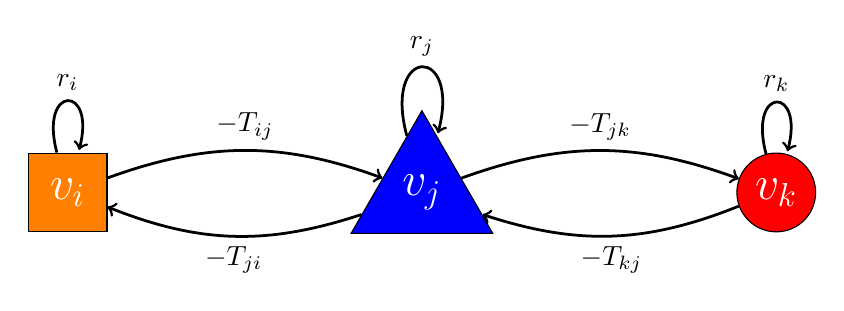
\begin{tikzpicture}[scale=1.8]
          % Define vertices
          \node[rectangle, draw, fill=orange, minimum size=1cm, text=white, font=\LARGE] (A) at (0,0) {$v_i$};
          \node[regular polygon, regular polygon sides=3, draw, fill=blue, minimum size=1cm, text=white, font=\LARGE] (B) at (2.5,0) {$v_j$};
          \node[circle, draw, fill=red, minimum size=1cm, text=white, font=\LARGE] (C) at (5,0) {$v_k$};

          % Draw edges
          \draw[line width=1pt, ->] (A) edge[bend left=20] node[above] {$-T_{ij}$} (B);
          \draw[line width=1pt, ->] (B) edge[bend left=20] node[below] {$-T_{ji}$} (A);
          \draw[line width=1pt, ->] (B) edge[bend left=20] node[above] {$-T_{jk}$} (C);
          \draw[line width=1pt, ->] (C) edge[bend left=20] node[below] {$-T_{kj}$} (B);
        
          % \draw[line width=1pt, black, dotted] (A) -- (-0.6,-0.9);
          % \draw[line width=1pt, black, dotted] (A) -- (0.6,-0.9);
          % \draw[line width=1pt, black, dotted] (C) -- (4.6,-0.9);
        
          % Draw self-edges.
          \draw[line width=1pt, ->,out=60,in=120,looseness=8] (A) edge[loop above] node {$r_i$} ();
          \draw[line width=1pt, ->,out=60,in=120,looseness=8] (B) edge[loop above] node {$r_j$} ();
          \draw[line width=1pt, ->,out=60,in=120,looseness=8] (C) edge[loop above] node {$r_k$} ();
        \end{tikzpicture}
\end{document}